\chapter{Design and Implementation}

In this project, the performance of IEEE 802.11b will be examined through simulation using NS-3. NS-3 is a discrete-event network simulator for Internet systems and is an open source software licensed under the GNU GPLv2 license~\cite{ns32015}. NS-3 is programmed in C++, but it has a feature for binding with Python. We have created a Python script to plot the result from NS-3. The script along with the main NS-3 application is automatically triggered through a shell script we made. Thus, it makes the simulation setup faster.

The infrastructured WLAN network with one AP is selected for this simulation and N-number of nodes. The topology of this network is depicted in Figure~\ref{fig:network-topology}.

\begin{figure}[H]
    \centering
    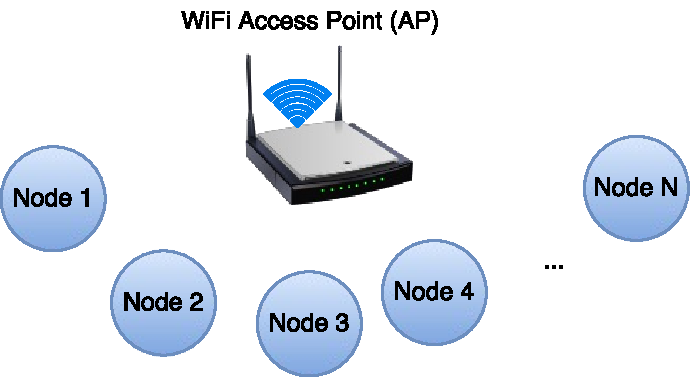
\includegraphics[width=0.6\textwidth]{figures/network-topology}
    \caption{Infrastructured WLAN topology with 1 AP and N-clients}
    \label{fig:network-topology}
\end{figure}

In order to build WiFi simulation in NS-3, first, we can make abstraction of the modules based on network layers just like in the OSI model. This is quite helpful when we start writing NS-3 program and also when we make a modification to the program. As a start, we define parameters of the simulation either define statically or dynamically by reading input arguments from users. Then, we specify the number of nodes (stations) and AP that will be used in the simulation. This can be done by using NodeContainer class.

After creating the containers, the physical layer (PHY) configuration has to be added to the containers. YansWifiPhyHelper and YansWifiChannelHelper are the NS-3 helpers that can be used to configure IEEE 802.11b standard. Here we can set the propagation loss model for the simulation.

For data link layer, the MAC parameter configurations can be added to select the  data rate offered by the standard. The default value of this configuration is 11 Mbps with Constant Rate mode. We also specify SSID and MAC address of the nodes and AP in this step.

One of the most important configurations used in this project is the mobility configuration. There are several mode that can be selected for simulation, such as constant mobility model, which is static, and 2D random walk model, which is dynamic. Using constant mobility model, we have created two different scenarios for placing the nodes, one is uniformly distributed across a circular path, and one is randomly distributed within a disc shape. For the circular path, we use a custom function to generate exact location of the nodes so that the nodes have the same relative distance to AP. Note that the AP is placed in the center of the circle. For the randomly distributed disc, we use a built-in NS-3 class, i.e. RandomDiscPositionAllocator, that is used to allocate random positions within a disc according to a given distribution for the polar coordinates of each node with respect to the provided center of the disc~\cite{ns32016}. 

The next step is configuring the network layer. We configure and assign IP addresses to the devices by using InternetStackHelper and Ipv4AddressHelper.

After configuring network layer, the next step is to configure transport layer. We use TCP for the simulation and set the AP as a transmission sink. Thus, all hosts try to send the data as much as possible to the sink during simulation time. Communication between AP and each node is established through a different port to prevent delay in case of the busy port. The traffics are generated with OnOff mechanism that follows On/Off pattern. The duration of ON state is equal to simulation time whereas the duration of OFF state is 0. This causes the packet generated constantly in each node.

It is interesting to see why TCP packets are used for this simulation. In contrast with UDP, TCP has a better mechanism to reduce the number of packet loss due to collision by performing three-way handshake. Thus, throughput calculation is more accurate than using UDP.

The effect of RTS/CTS mechanism is also evaluated in the simulation. By setting the RTS/CTS threshold value, we can either enable or disable the use of RTS/CTS packets. As the default RTS/CTS threshold value is set to 150 bytes and the payload size is 1024 bytes, RTS/CTS mechanism will be used. To disable this, the threshold value should be set above the payload size. For instance, the threshold value can be set to 2000 bytes.

To measure the throughput, FlowMonitor, which is a built-in class in NS-3, is used. Essentially, FlowMonitor is utilized to monitor packet flows in the simulation. The throughput itself is defined as the sum of data received by the sink, in this case, the AP, divided by transmission time. Note that transmission time is the difference between timestamp of last packet and timestamp of first packet. However, NS-3 simulator will give the same result once we run the same set of simulation. One of the solutions is by adding randomness using seed functions. This can be done by using the RngSeedManager class. 

To recap, the scenario that will be evaluated in this project are:
\begin{enumerate}
\item Throughput vs Node placement and mobility
\item Throughput vs Payload size
\item Throughput vs the use of RTS/CTS
\end{enumerate}